% Why prediction is important?
\label{sec:prediction}

\subsection{Overview}
%\begin{figure*}[!htb]
\label{sec:predictoverview}

\begin{figure}[!h]
\begin{center}
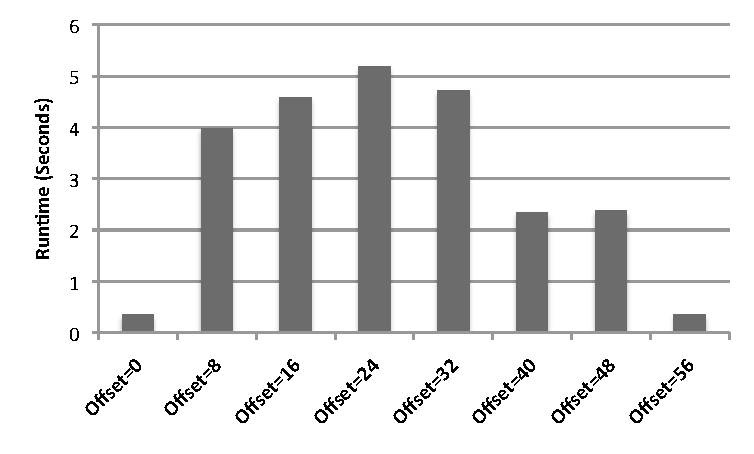
\includegraphics[width=3.3in]{fig/perfsensitive}
\end{center}
\caption{
Inside \texttt{linear\_regression} benchmark,
performance is sensitive to the offset between starting address of the false sharing object 
and the starting of cache line 
\label{fig:perfsensitive}}
\end{figure}

Occurrence of false sharing highly depends on 
alignments between objects and corresponding cache lines.
We can see an example in Figure~\ref{fig:perfsensitive}, one benchmark evaluated in
Section~\ref{sec:evaluation}. 
For this \texttt{linear\_regression} benchmark,
when the offset of starting address between false sharing object and corresponding cache lines 
is $0$ or $56$ bytes, 
there is no false sharing problem in this benchmark. 
When the offset is $24$ bytes, we see the most severe performance effect caused 
by false sharing problem. 
The performance difference between these two can be as large as $15\times$.
None of existing detection tools considers this possibility caused by alignments. 
Thus, existing tools can only report those manifested false sharing at best. 
For this example, they may miss a very severe false sharing problem if the offset of starting 
address is actually $0$ bytes or $56$ bytes in their test environment.
\Predator{} overcomes this shortcoming by predicting potential false sharing accurately. 

\begin{figure*}
\begin{center} 
\subfigure[No false sharing]{%
   \label{fig:nofs}
   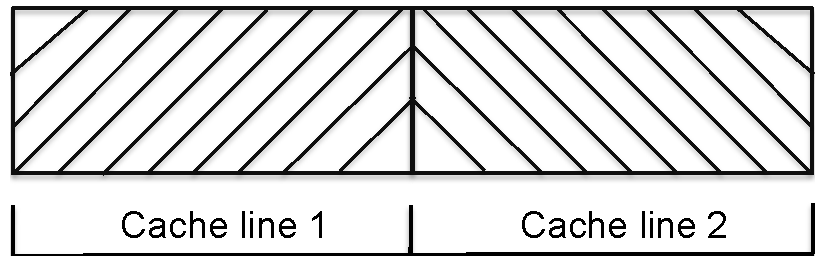
\includegraphics[width=0.24\textwidth]{fig/Potential1}
}%
\hspace{30pt}
\subfigure[False sharing with larger cache size]{%
   \label{fig:fslarger}
   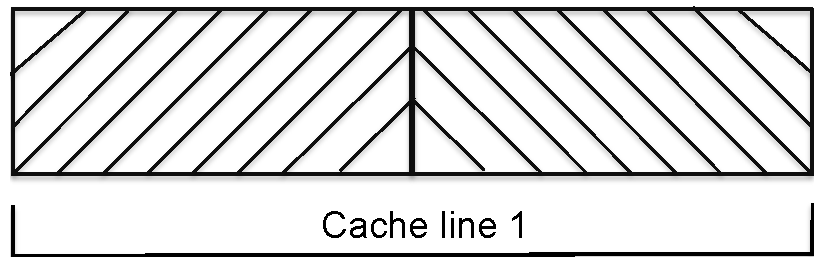
\includegraphics[width=0.24\textwidth]{fig/Potential2}
}%
\hspace{30pt}
\subfigure[False sharing with different alignment]{%
   \label{fig:fsnoalignment}
   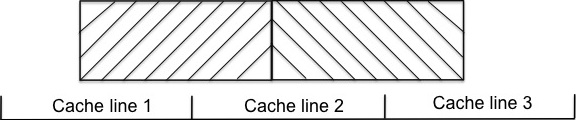
\includegraphics[width=0.36\textwidth]{fig/Potential3}
}%
\end{center}
%\includegraphics{fig/potential.pdf}
\caption{Manifestness of false sharing changes under different environment}
\label{fig:potentialfalsesharing}
\end{figure*}

The prediction of \Predator{} focuses on {\it potential false sharing}, the type of
false sharing that does not 
manifest in current execution but may appear and greatly affect programs' performance
in a slightly different environment.

Figure~\ref{fig:potentialfalsesharing} shows a simplified example.
In this figure, two rectangles with different patterns
represents two portions of the same object. 
In Figure~\ref{fig:nofs}), there is no false sharing when thread T1 only updates 
``cache line 1'' and T2 only updates ``cache line 2''.
However, false sharing appears in one of the following cases even with the same
access pattern. 

\begin{itemize}
\item
Doubling cache line size (Figure~\ref{fig:fslarger}). When the size of a
cache line doubles,
T1 and T2 access the same cache line. False sharing occurs in this case.

\item
Different starting address of an object. 
When the starting address of this object is not aligned with the starting address of 
the first cache line, 
then T1 and T2 can update the second cache line simultaneously, 
which causes false sharing (Figure~\ref{fig:fsnoalignment}). 
%When some dynamic property changes the starting address of this object so that it 
%is not aligned with the starting address of the first cache line, 
\end{itemize} 

\Predator{} predicts whether there are false sharing 
in any of these two cases, which can
be caused by those dynamic properties discussed in Section~\ref{sec:intro}.
For example, all dynamic properties except change of cache line size 
can lead to different starting address of an object. 
Thus, predicting false sharing in these two cases actually 
explores many possibilities caused by all dynamic properties.

\subsection{Basic Workflow of Prediction}
\label{sec:predictionmechanism} 

Similar to the detection part, 
\Predator{} only precticts those potential false sharing that can 
cause performance problem.
The implementation is based on
two important observations. First, only accesses to 
adjacent cache lines can form potential false sharing, 
i.e., introducing cache invalidations when cache line size
or an object's starting address changes.
Second, false sharing can greatly degrade performance when 
there are a large amount of cache invalidations.

Based on these two observations, \Predator{} develops 
the following workflow to capture potential false sharings.
Those optimizations listed in Section~\ref{optimization} also apply
here, although we do not repeat these optimizations in
this whole section.

\begin{enumerate}
\item
Track writes on different cache lines. 

\item
When the number of writes to a cache line $L$ reaches {\it Tracking-Threshold},
track the detailed read and write accesses for every word on both current cache line 
and adjacent cache lines. 

\item
When the number of writes to a cache line $L$ reaches a second threshold (called as
{\it Predicting-Threshold}), 
identify potential false sharing by evaluating these word accesses on $L$ and 
its adjacent cache lines. Section ~\ref{sec:evaluatingfs} describes the evaluation method.
%Since this threshold is used to trigger the prediction process, we call it
%prediction-trigger threshold.

\item
If a potential false sharing is found, continue to track cache line invalidations
to confirm it. Section~\ref{sec:tracking} discusses the details.
Otherwise, go back to Step 2 to track more detailed accesses.
 
\end{enumerate}

\subsection{Evaluating Potential False Sharing}
\label{sec:evaluatingfs}
%For simplicity, \Predator{} do not evaluate potential false sharing if a cache line 
%has actual false sharing.
To describe easily, we first introduce a {\it virtual line} concept:
A virtual line is {\it a memory range with certain size}.
When the number of writes on a cache line $L$ reaches the {\it Predicting-Threshold},
\Predator{} evaluates potential false sharing by computing the number of possible cache 
invalidations on a virtual line. Specifically, if the number of cache
invalidations is larger than the average number of accesses
on each word of $L$, a potential false sharing is considered to
be identified by \Predator{}.

\Predator{} computes the number of possible cache invalidations based on a 
similar observation as detection~\ref{sec:overview}: 
{\it if a thread writes a virtual line after other threads 
have accessed the same virtual line, this write operation most likely causes at least a cache 
invalidation}. 
However, it is impossible to know exactly how many cache invalidations occur on a virtual
line without knowing actual access sequence of different threads.  
\Predator{} makes a conservative assumption that 
accesses from different threads are issued in an interleaving way and
continues to verify the evaluation result after prediction (See Section~\ref{sec:tracking}).
This ensures we don't miss any potential false sharing as well as 
not reporting false positives.

To compute possible cache invalidations, a way is to compute possible 
cache invalidations of $L$ word by word and then sum up all possible cache invalidations 
of every word in cache line $L$. 
However, it is slow and can largely over-estimate possible cache invalidations.
To address this problem, \Predator{} only cares about those cache invalidations caused by
{\it hot accesses}. A hot access in a cache line refers to the word whose number of read or write accesses 
is larger than the averaged number of accesses on each word in the same cache line.
For every hot access $X$ in cache line $L$, \Predator{} searches another
hot access $Y$ in $L$'s previous cache line or next cache line satifying with
the following conditions: 

\begin{itemize}
\item
$X$ and $Y$ fall into the same virtual line. 

\item
One of $X$ and $Y$ is a write access.

\item 
$X$ and $Y$ are issued by different threads.

\end{itemize}

Whenever it finds an pair of $X$ and $Y$, 
\Predator{} computes the number of cache invalidations caused by $X$ and $Y$.
Based on our observation and conservative assumption,
this pair of $X$ and $Y$ should at least cause cache invalidations 
larger than the average number of accesses to each word of $L$ since both of them 
are hot accesses.
Thus \Predator{} identifies a potential false sharing place and stops searching.

Note that \Predator{} has different specification for a virtual line in
different scenarios. 
For the case of double cache line size, a virtual line has twice
 as large as original size and forms by two original 
continuous cache lines starting with the even number index of cache line, 
e.g. $2*i$ and $2*i+1$ cache line.
For the case of starting address change,
a virtual line still has the same cache line size as orignal lines, but
different starting address.
For instance, a virtual line can be formed by 1st word to 64th word, or 2nd word to 65th word.
Although making such a virtual line can never be a real line in hardware due to unaligned starting
address, this mechanism allows to accurately simulate the results of having different starting address of an
object on a real cache line.


\subsection{Verifying Potential False Sharing}
\label{sec:tracking}

\Predator{} verifies potential false sharing by tracking 
cache invalidations on those virtual lines. 

For potential false sharing caused by double cache line size, as described in
last section~\ref{sec:evaluatingfs}, a virtual line is composed of 
cache line with index $2*i$ and $2*i+1$. \Predator{} verifies cache invalidations
on a virtual line on which false sharing has been discovered.

However, for the case with starting address change, 
two hot accesses with distance less than cache line size 
can form multiple virtual lines. 
So there is an additional step to determine which virtual line to be tracked.

\begin{figure}
\begin{center} 
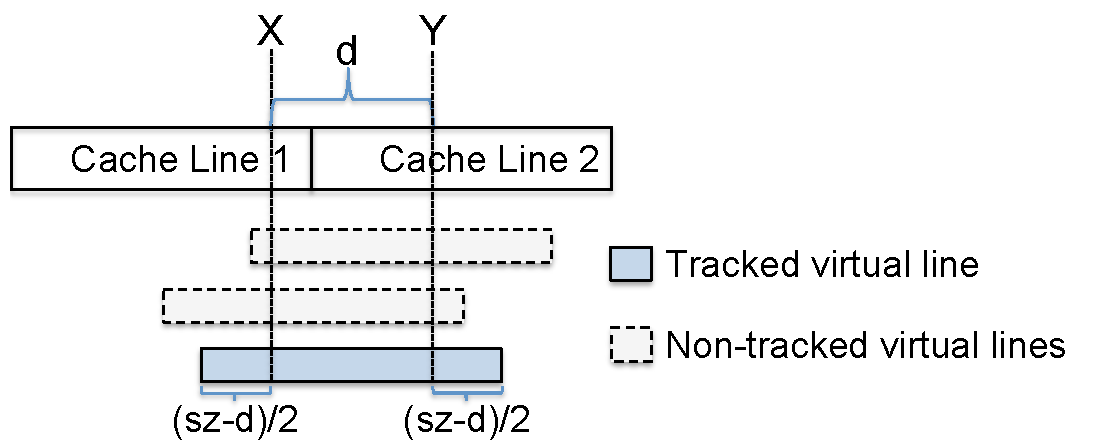
\includegraphics[width=3.3in]{fig/trackpotential}
\end{center}
\caption{Determining a virtual line with size $sz$ according to hot accesses.}
\label{fig:trackpotential}
\end{figure}

Given two words having hot accesses showed in Figure~\ref{fig:trackpotential}, 
\Predator{} leaves the same space before $X$ and after $Y$ in determining a virtual line. 
That is, the virtual line starting 
at location $X-((sz-d)/2)$ and ending at $Y+((sz-d)/2)$ is tracked. 
This adjustment allows to track more possible cache invalidations caused by
accesses to $X$ and $Y$ and adjacent accesses.
Since adjusting the starting address of a virtual line has the same effect of
adjusting the starting address of an object in detecting false sharing, thus
all cache lines related to the same object must be adjusted in the same time.
\Predator{} then tracks cache invalidations based on these adjusted virtual lines.
\begin{comment}
In the end, \Predator{} can report to users how to adjust the starting address of an
object can manifest all hided false sharing.
\end{comment}
